% Workshop paper (~4 pages content). Compile on Overleaf.
% To retarget a venue, swap \documentclass for the venue style (e.g. neurips_2026.sty) and
% move the two figure PDFs in figures/ accordingly. No venue-specific macros are used below.
\documentclass[11pt]{article}
\usepackage[margin=1in]{geometry}
\usepackage{graphicx}
\usepackage{booktabs}
\usepackage{amsmath}
\usepackage{amssymb}
\usepackage{hyperref}
\usepackage{xcolor}
\usepackage{caption}
\captionsetup{font=small}
\hypersetup{colorlinks=true, linkcolor=black, citecolor=black, urlcolor=blue}

\title{\textbf{Attention-Output Variance Is a Symptom, Not a Cause,\\ of Length-Generalization Failure}}
\author{Anonymous\\ \small(workshop submission)}
\date{}

\begin{document}
\maketitle

\begin{abstract}
Explanations of why transformers fail to generalize to longer sequences increasingly point to a single
internal statistic. A prominent recent candidate is \emph{attention-output variance}, which collapses as
sequences grow; the accompanying prescription is to stabilize it with a post-attention layer
normalization. We take the position that this statistic is a \emph{symptom} rather than a lever, and test
it directly. In a controlled study spanning positional encoding $\{\text{NoPE},\text{RoPE}\}$, the
variance-stabilizing normalization $\{\text{off},\text{on}\}$, and three tasks $\{$argmax retrieval, flag
retrieval, addition$\}$ (four seeds for the order-invariant tasks, two for addition), we first confirm the phenomenon -- the variance collapses with
length in every baseline -- and verify that the normalization does what it claims, holding the
downstream variance essentially constant across length. Yet it does not improve length generalization:
its per-token benefit at long sequences ($50\times$ the training length) is $\le 0$ in every
order-invariant cell (four seeds) and it is consistently \emph{harmful} under RoPE (up to $-0.08$,
negative in all four seeds); it also fails to rescue an order-dependent task (addition).
Stabilizing the variance therefore leaves -- and under RoPE worsens -- the behavior it was meant to fix.
We then localize the operative variable: on tasks where the correct source token is known, attention mass
on that token predicts accuracy almost perfectly ($r=0.97$) while variance is a far weaker correlate
($r=0.59$), and the fix fails to restore this attention (reducing it under RoPE). We conclude that
attention-output variance is a symptom, not a cause; the driver is attention dispersion off the correct
source. We argue that interventions motivated by an internal diagnostic should be validated against the
target behavior directly and across positional encodings. Code, data, and a pre-registration are released.
\end{abstract}

\section{Introduction}
Transformers trained on short sequences often fail on longer ones, and a natural research instinct is to
find the internal quantity responsible -- a statistic that collapses, saturates, or drifts as length
grows, and whose repair would restore generalization. Attention-output variance is an appealing instance
of this template: the variance of attention-module outputs shrinks with length, producing a train/test
distribution shift, and a layer normalization applied after the attention output restores the variance
scale~\cite{vanishingvariance}. The story has a clean causal shape -- diagnose the statistic, normalize
it, recover the behavior. A competing account instead blames \emph{attention dispersion} -- attention
flattening as more tokens compete -- and prescribes sharpening the attention distribution. The two
accounts implicate different statistics and prescribe different fixes; they have not, to our knowledge,
been compared head-to-head.

We take a skeptical position and adjudicate: an internal statistic that \emph{co-occurs} with a failure is
not necessarily its \emph{cause}, and repairing the statistic is a direct test of that distinction. We
operationalize the most concrete form of the variance hypothesis -- a post-attention layer normalization
-- and ask whether stabilizing the variance restores length generalization, across two axes that
existing evaluations of this idea leave fixed: the positional encoding, and whether the task is
order-dependent.

\paragraph{Contributions.}
\begin{itemize}\itemsep2pt
\item A pre-registered study (positional encoding $\times$ variance fix $\times$ task, up to four seeds)
that reproduces variance collapse, verifies the fix stabilizes the downstream variance, and then isolates
the statistic's causal role.
\item Evidence that stabilizing attention-output variance does \emph{not} improve length generalization:
the fix's benefit at long sequences is $\le 0$ across order-invariant tasks, despite the variance being
demonstrably stabilized.
\item A positional-encoding interaction: the fix is neutral under NoPE but \emph{harmful} under RoPE
(up to $-0.08$ per-token at $50\times$ length, negative in all four seeds) -- an axis absent from prior
evaluations of the idea.
\item A positive identification of the driver: attention mass on the correct source token predicts
accuracy ($r=0.97$) far better than variance ($r=0.59$); the fix leaves it unrestored and, under RoPE,
reduces it -- a mechanistic account of the RoPE harm.
\item The resulting stance: attention-output variance is a symptom, not a cause, of
length-generalization failure; the operative variable is attention dispersion off the correct source, and
diagnostic-motivated interventions need behavioral validation.
\end{itemize}

\section{Related work}
Explanations of length-generalization failure increasingly single out one internal statistic that
degrades with length. Two are prominent, and they disagree about which:

\paragraph{The variance-collapse account.} \cite{vanishingvariance} identifies attention-output variance
collapse as the driver and proposes a post-attention layer normalization as the remedy, evaluated on
order-invariant retrieval tasks with positional encodings removed to isolate the variance effect.

\paragraph{The attention-dispersion account.} A separate line argues that the operative quantity is
attention concentration: as more tokens compete, softmax attention flattens, and length generalization
fails. \cite{nopeentropy} ties the attention-entropy inflection to the length-generalization inflection
(and reports an attention-sharpening intervention that helps NoPE but not RoPE); scalable-softmax
sharpens attention by scaling logits by $\log n$ and improves long-context retrieval~\cite{ssmax}; and
sparse attention that limits dispersion generalizes to far longer sequences~\cite{sparselong}.

These accounts prescribe different fixes (normalize the variance vs.\ sharpen the attention), and to our
knowledge have not been compared head-to-head. We adjudicate: we adopt the variance remedy exactly as
proposed~\cite{vanishingvariance}, and measure its behavioral effect while directly tracking the
attention-dispersion quantity, on identical tasks, across positional encodings, and on an
order-dependent task.

\paragraph{Positional encoding and downstream components.} We treat the positional encoding as a
first-class variable rather than removing it. This matters because components outside attention interact
with RoPE: \cite{fope} shows that linear layers and activation functions cause ``spectrum damage'' to
RoPE's periodicity and harm length generalization, and \cite{postnorm} studies how post-attention
normalization reshapes attention sharpness -- context for the positional-encoding interaction we report.

\section{The intervention and hypothesis under test}
We test the representative variance-stabilizing operator: a layer normalization applied to the attention
output $z=W_O\,\mathrm{Attn}(x)$ \emph{before} the residual addition, i.e. $h \leftarrow h +
\mathrm{LN}(z)$ in place of $h \leftarrow h + z$~\cite{vanishingvariance}. If attention-output variance
collapse is the operative cause of length-generalization failure, then holding the downstream variance
constant across length should restore extrapolation. We test this where prior evaluations do not vary:
under both NoPE and RoPE, and on an order-\emph{dependent} task where token position is load-bearing.

\section{Experimental design}
\paragraph{Grid.} We cross positional encoding $\{\text{NoPE},\text{RoPE}\}$, the fix
$\{\text{off},\text{on}\}$, and three tasks; four seeds per cell for the order-invariant tasks and two
for addition.

\paragraph{Tasks.} \emph{argmax retrieval} and \emph{dictionary lookup} are the order-invariant
retrieval tasks used to motivate the variance hypothesis; we additionally use \emph{flag retrieval}
(output the single marked value in a sequence -- an order-invariant task a small model masters reliably)
and \emph{reversed decimal addition} as an order-\emph{dependent} contrast. Symbols use disjoint
vocabularies large enough that long sequences draw distinct tokens; answers are supervised token-wise.
(Dictionary lookup did not reach our training-competence gate at this scale and is reported as untrained;
see Limitations.)

\paragraph{Model and training.} A 4-layer pre-norm decoder ($d{=}256$, 8 heads, MLP width $1024$),
trained with AdamW, batch $512$, warmup $+$ cosine schedule, on sequences of length $1\ldots 5$; we
evaluate to many times that length. The model is small by design: the variance effect is architectural
and should manifest most cleanly where collapse is severe.

\paragraph{Observables.} (1) \emph{per-token accuracy} vs.\ length (a graded metric; exact-match is an
all-or-nothing upper bound and is reported at the training length as a mastery check), and (2)
\emph{attention-output variance} vs.\ length, captured per layer both \emph{before} the fix (the raw
collapse) and \emph{after} it (to confirm the fix stabilizes the downstream variance).

\paragraph{Pre-registration and validity gates.} Before viewing outcomes we fixed: (i) a cell is
\emph{informative} only if its training-length exact-match $\ge 0.8$; (ii) the fix's benefit is measured
at the longest length where the \emph{no-fix} baseline actually breaks (per-token $<0.9$), so a task that
never breaks cannot masquerade as a null; and (iii) we must reproduce the variance-collapse phenomenon
before interpreting any null. Our normalization is exactly the proposed remedy, and NoPE matches the
positional-encoding-free setting in which the variance hypothesis was originally isolated.

\section{Results}

\subsection{The variance collapse is present, and the fix stabilizes it}
In every baseline, deep-layer attention-output variance falls with length (Table~\ref{tab:main}, the
``pre'' side of the variance column collapses to $0.20$--$0.49$ of its train-length value at $50\times$;
Figure~\ref{fig:var}). With the fix on, the downstream (post-normalization) variance is held essentially
constant across length (``post'' $\approx 1.0$ in every order-invariant cell). The intervention therefore
does exactly what it is designed to do -- any null below is not a failure of the fix to act, but a failure
of that action to matter.

\subsection{Stabilizing the variance does not improve length generalization}
All cells master the training length (exact-match $=1.00$) and degrade with length
(Figure~\ref{fig:acc}, Table~\ref{tab:main}). On the two order-invariant tasks the fix never improves
extrapolation: its per-token benefit at long length is $\le 0$ in every cell. The variance is stabilized;
the behavior is not.

\subsection{A positional-encoding interaction}
The sign is not uniform across positional encodings. Under NoPE the fix is approximately neutral (argmax
$-0.013$, negative in $2/4$ seeds); under RoPE it is consistently and substantially \emph{harmful}
(argmax $-0.033$, flagret $-0.061$, both negative in all four seeds; flagret/NoPE is also
strongly negative, $-0.081$). Because the variance hypothesis was isolated with positional encodings
removed, this interaction is invisible in that setting; it means the recommended intervention can
actively degrade the most widely deployed positional encoding.

\subsection{The order-dependent contrast}
Reversed addition is mastered at the training length and then fails completely: exact-match is $0$ at
every extrapolation length, with and without the fix. The fix produces a cosmetic per-token bump under
NoPE while exact-match stays $0$ -- a reminder that a graded metric alone can mislead -- and is neutral
under RoPE. No configuration recovers usable length generalization.

\subsection{The operative variable: attention on the correct source}
If variance is not the lever, what is? For the order-invariant tasks we know the input position holding
the answer, so we measure, per layer at the answer-query position, the attention mass placed on that
correct source token. Across length and both positional encodings, this quantity predicts per-token
accuracy almost perfectly (mean within-cell Pearson $r=0.97$ over the 16 baseline runs;
Figure~\ref{fig:causal}, left), whereas the variance-collapse ratio is a far weaker predictor
($r=0.59$ pooled; $r\approx0.3$ for flagret; Figure~\ref{fig:causal}, right). The failure is thus
localized to \emph{attention}: as sequences grow, attention on the correct source disperses (from
$\approx1.0$ toward chance) and accuracy falls with it. Moreover, the fix does not restore this attention
at long length, and under RoPE it \emph{reduces} it (argmax $0.25\!\to\!0.07$, flagret
$0.016\!\to\!0.010$ at $50\times$) -- a mechanistic account of why the fix is harmful under RoPE. We frame
this as strong correlational localization, not proof: that attention on the token one must copy predicts
copying it is expected; the informative content is that it is a \emph{far} better predictor than variance
and that the fix moves it the \emph{wrong} way.

\begin{table}[t]
\centering\small
\caption{Order-invariant tasks (argmax retrieval, flag retrieval), four seeds. Per-token accuracy at
multiplicative lengths ($1\times$ = training length); the deep-layer attention-output variance-collapse
ratio (var@$50\times$/var@$1\times$) \emph{before} $\to$ \emph{after} the fix (``after'' $\approx 1.0$ =
the fix stabilizes the downstream variance as intended); and the fix's \emph{paired per-seed} benefit at
the $50\times$ break point, $\Delta$ [min,\,max] with the count of seeds in which the fix hurts. All cells
have training-length exact-match $=1.00$. Every order-invariant $\Delta\le 0$; under RoPE the fix hurts in
all four seeds.}
\label{tab:main}
\begin{tabular}{llcccc c c}
\toprule
task & PE\,/\,fix & $1\times$ & $3\times$ & $10\times$ & $50\times$ & var: pre$\to$post & $\Delta$@$50\times$ \\
\midrule
argmax  & NoPE, off & 1.00 & 0.98 & 0.83 & 0.59 & $0.33\to0.33$ & \\
        & NoPE, on  & 1.00 & 0.97 & 0.80 & 0.58 & $0.20\to0.99$ & $-0.013$ [$-.035,+.004$], 2/4\\
        & RoPE, off & 1.00 & 0.95 & 0.77 & 0.60 & $0.27\to0.27$ & \\
        & RoPE, on  & 1.00 & 0.96 & 0.67 & 0.57 & $0.45\to1.00$ & $-0.033$ [$-.066,-.008$], 4/4\\
\midrule
flagret & NoPE, off & 1.00 & 0.94 & 0.67 & 0.60 & $0.47\to0.47$ & \\
        & NoPE, on  & 1.00 & 0.88 & 0.62 & 0.52 & $0.49\to1.00$ & $-0.081$ [$-.109,-.043$], 4/4\\
        & RoPE, off & 1.00 & 0.99 & 0.65 & 0.56 & $0.48\to0.48$ & \\
        & RoPE, on  & 1.00 & 0.96 & 0.53 & 0.50 & $0.43\to1.00$ & $-0.061$ [$-.074,-.047$], 4/4\\
\bottomrule
\end{tabular}
\\[3pt]
{\footnotesize Order-\emph{dependent} contrast (addition, two seeds): mastered at $1\times$
(exact-match $1.00$) then fails at every extrapolation length (exact-match $0$ throughout, with and
without the fix). The fix gives only a cosmetic per-token bump under NoPE ($+0.047$ at $20\times$, while
exact-match stays $0$) and is neutral under RoPE ($-0.004$). No configuration recovers usable
length generalization.}
\end{table}

\begin{figure}[t]
\centering
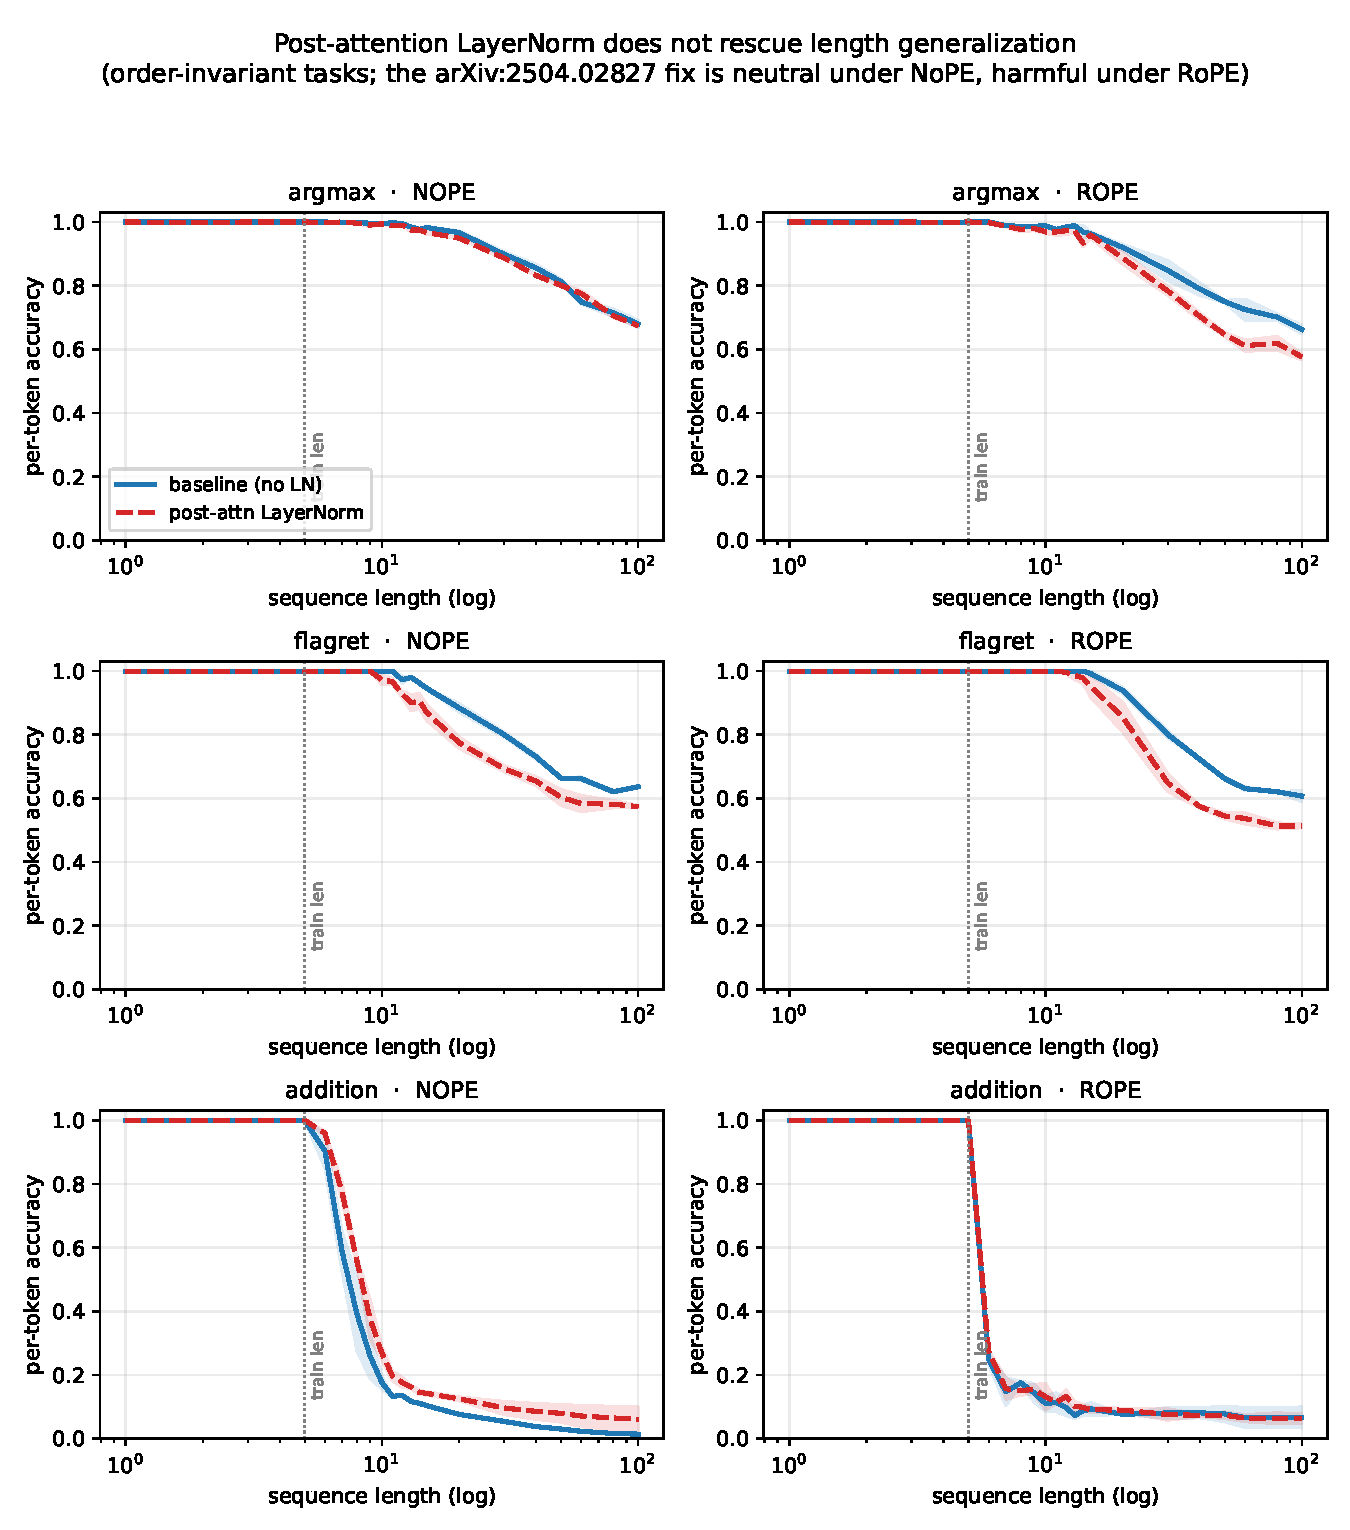
\includegraphics[width=\linewidth]{figures/fig_accuracy_vs_length.pdf}
\caption{Per-token accuracy vs.\ sequence length (log axis; to $50\times$ the training length for the
order-invariant tasks), baseline (solid) vs.\ variance-stabilizing normalization (dashed), mean over four
seeds (bands: min--max). The fix lies at or below the baseline in every panel and clearly below --- with
separated bands --- under RoPE. Addition (bottom) fails off a cliff regardless of the fix.}
\label{fig:acc}
\end{figure}

\begin{figure}[t]
\centering
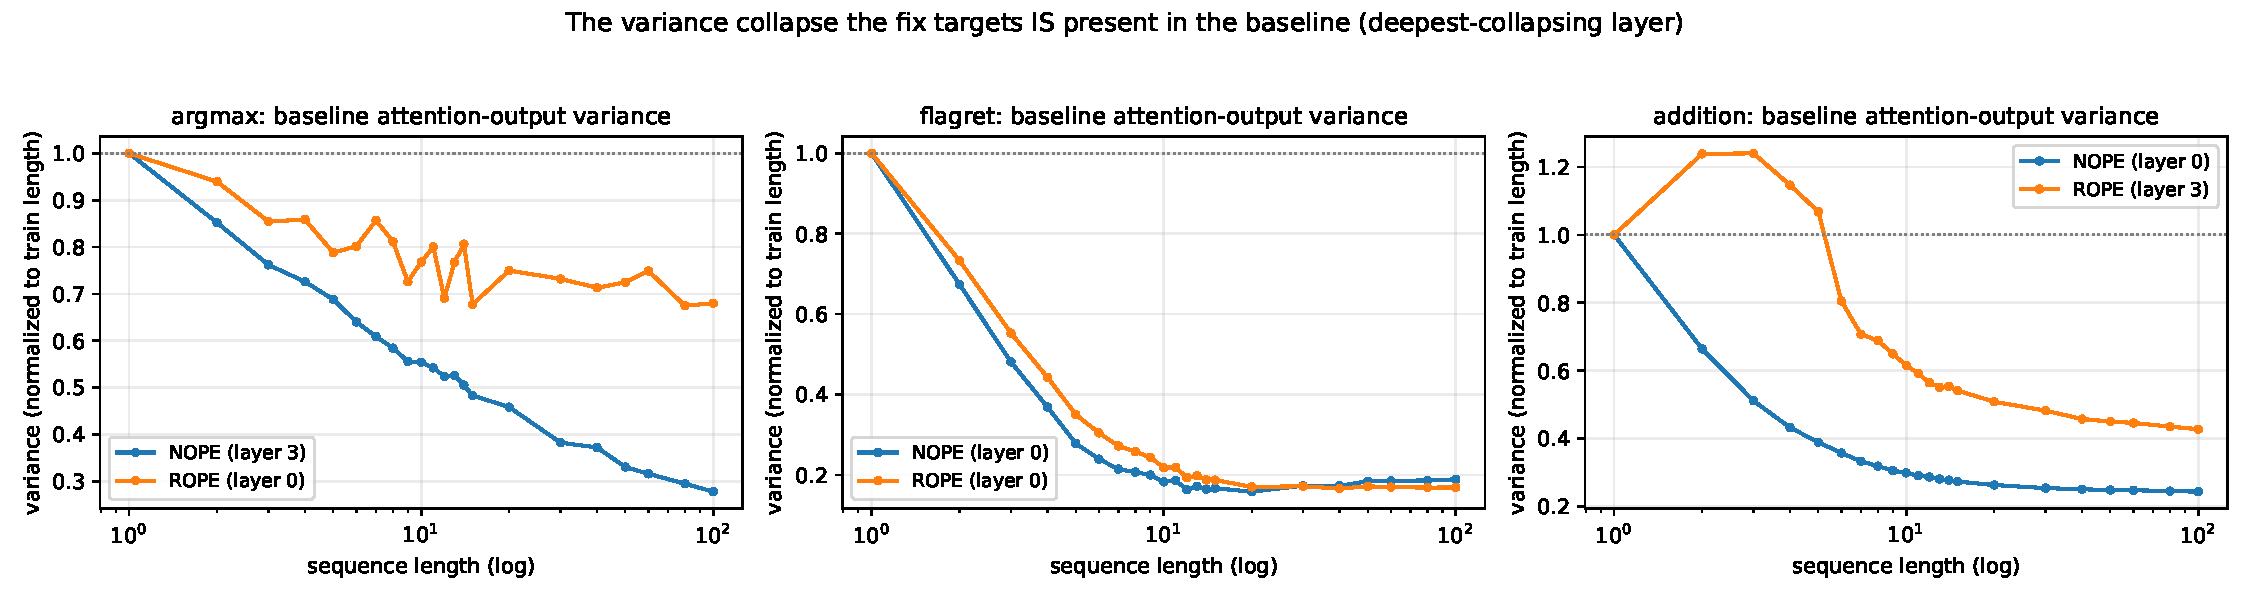
\includegraphics[width=\linewidth]{figures/fig_variance_collapse.pdf}
\caption{Baseline attention-output variance (deepest-collapsing layer, normalized to the training
length) falls with length on every task -- the phenomenon the intervention targets is present.}
\label{fig:var}
\end{figure}

\begin{figure}[t]
\centering
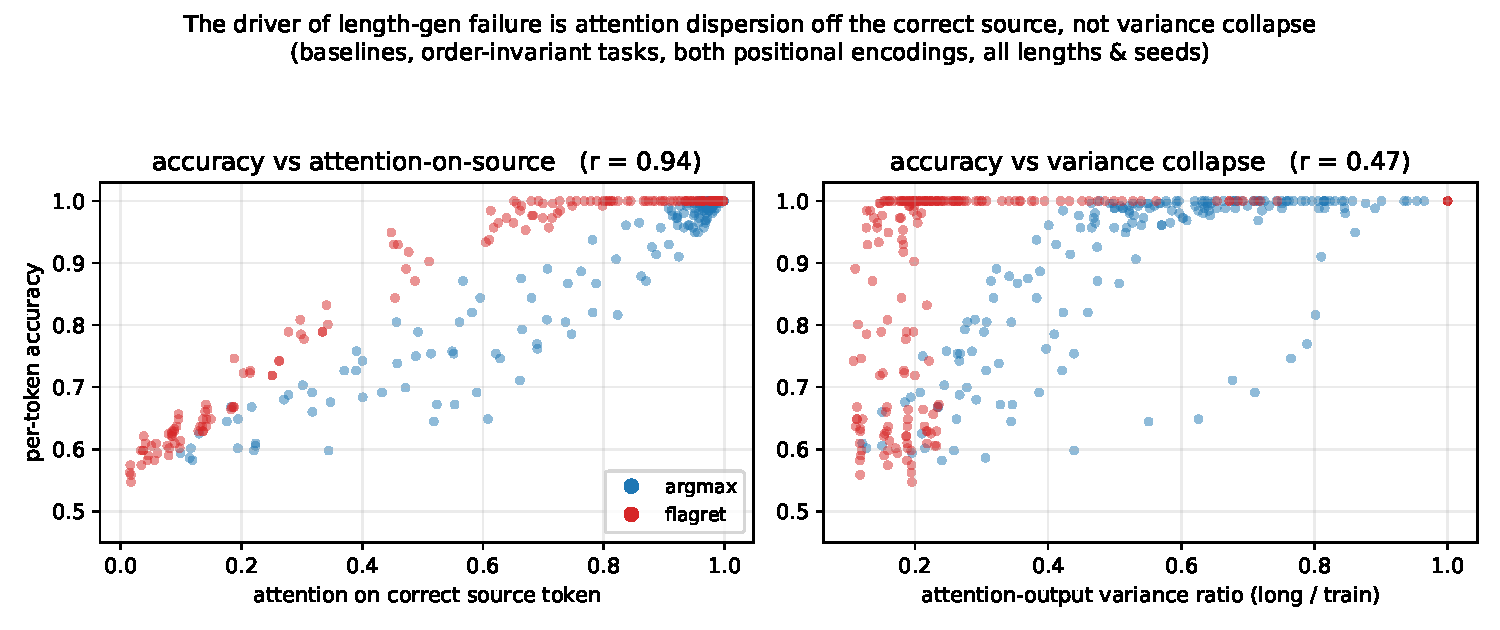
\includegraphics[width=\linewidth]{figures/fig_causal.pdf}
\caption{Pooled over baseline runs, lengths, and seeds. \emph{Left:} per-token accuracy vs.\ attention on
the correct source token -- a tight relationship ($r=0.94$). \emph{Right:} accuracy vs.\ the
attention-output variance ratio -- diffuse ($r=0.47$), with flagret (red) a near-vertical smear. The
operative variable is attention dispersion off the correct source, not variance.}
\label{fig:causal}
\end{figure}

\section{Discussion}
Across three tasks, two positional encodings, and up to four seeds, an intervention that demonstrably
stabilizes attention-output variance does not improve length generalization, and under RoPE degrades it.
The most economical reading is that the variance signature is a \emph{symptom} that co-occurs with the
failure rather than its operative cause. Our attention measurement adjudicates the two accounts of
Section~2 in favor of \emph{dispersion}: attention on the correct source predicts accuracy ($r=0.97$),
variance does not ($r=0.59$), and the variance remedy leaves attention unrestored.

\paragraph{Why variance can collapse without mattering.} The attention output is a convex combination of
value vectors, $z=\sum_j a_j v_j$ with $\sum_j a_j=1$. As attention spreads over more competitors, $z$
tends toward an average and its variance shrinks by a law-of-large-numbers effect -- \emph{regardless} of
whether the correct value is selected. Length generalization, however, depends on the \emph{selection}
($a_j$ concentrated on the right $j$), a property of the attention weights that a normalization of $z$
does not touch. Variance collapse and selection failure thus co-occur but are distinct; repairing the
former leaves the latter, which is what we observe.

\paragraph{The RoPE interaction.} That the fix \emph{hurts} under RoPE -- reducing attention on the
correct source -- is consistent with evidence that components outside attention damage RoPE's frequency
structure and its length generalization~\cite{fope}, and it nuances the finding that post-attention
normalization can resharpen attention~\cite{postnorm}: under RoPE, in our setting, that resharpening
reverses. It also matches the report that attention-sharpening behaves differently under RoPE than under
NoPE~\cite{nopeentropy}.

We do not claim variance is irrelevant everywhere, nor that no variance-based operator could help; we
claim, from this evidence, that attention-output variance is not a reliable lever for length
generalization, whereas attention dispersion is the operative variable. Practically: interventions
motivated by an internal diagnostic should be validated against the target behavior \emph{directly} and
\emph{across positional encodings}, because a fix that provably repairs the statistic can leave the
behavior unchanged and, under RoPE, worse.

\section{Limitations}
Our models are small (4 layers, $d{=}256$); the variance phenomenon has been documented on large models,
whereas we test the \emph{intervention} at small scale. We argue the setting is informative because the
effect is architectural and collapse is severe here, but we do not establish behavior at frontier scale,
and we do not reproduce a length-generalization \emph{benefit} for the fix in any cell -- we cannot
exclude that one emerges at larger scale or under a specific task construction. We test one
variance-stabilizing operator (post-attention layer normalization); other operators may differ. Our
identification of attention dispersion as the driver is \emph{correlational}: it localizes the failure and
shows the fix targets the wrong quantity, but the causal test (intervening to sharpen attention and
measuring whether length generalization recovers) is left to future work. Our accuracy is teacher-forced
per-token (an upper bound on free generation). Dictionary lookup did not reach
our competence gate at this scale and is reported as untrained rather than as a null. These bound the
generality of the stance to the settings we measure.

\section{Conclusion}
Attention-output variance collapse is real and reproducible, and a post-attention layer normalization
provably stabilizes it -- yet doing so does not improve length generalization on the tasks where the
variance hypothesis is motivated, and hurts under RoPE. In these settings, variance stabilization is
decoupled from length generalization: the statistic is a symptom, not a cause. We recommend that
variance-motivated interventions be validated against the target behavior directly and across positional
encodings.

\paragraph{Reproducibility.} Code, the full result file, the analysis script, and the pre-registration
(written before viewing outcomes) are released with the paper.

\bibliographystyle{plain}
\bibliography{references}
\end{document}
